% !TEX root = main.tex

\section{Результаты расчётов}

\begin{align*}
    M_{\min} &= 6.81; \\
    M_{\max} &= 12.41; \\
    R &= 5.6; \\
    \hat{\mu}(\vec{X}_n) &= 9.4872; \\
    S^2(\vec{X}_n) &= 1.2173.
\end{align*}

\noindent 
Интервальная групировка значений выборки при $m = 8$:
\[
    [6.81;7.51),	[7.51;8.21),	[8.21;8.91),	[8.91;9.61),	[9.61;10.31),
\]
\[
   [10.31;11.01),	[11.01;11.71),	[11.71;12.41]
\]



\section{Графики}

\subsection{Гистограмма и график функции плотности распределения вероятностей нормальной случайной величины с математическим ожиданием $\hat{\mu}$ и дисперсией $S^2$}


\begin{figure}[h]
    \centering
    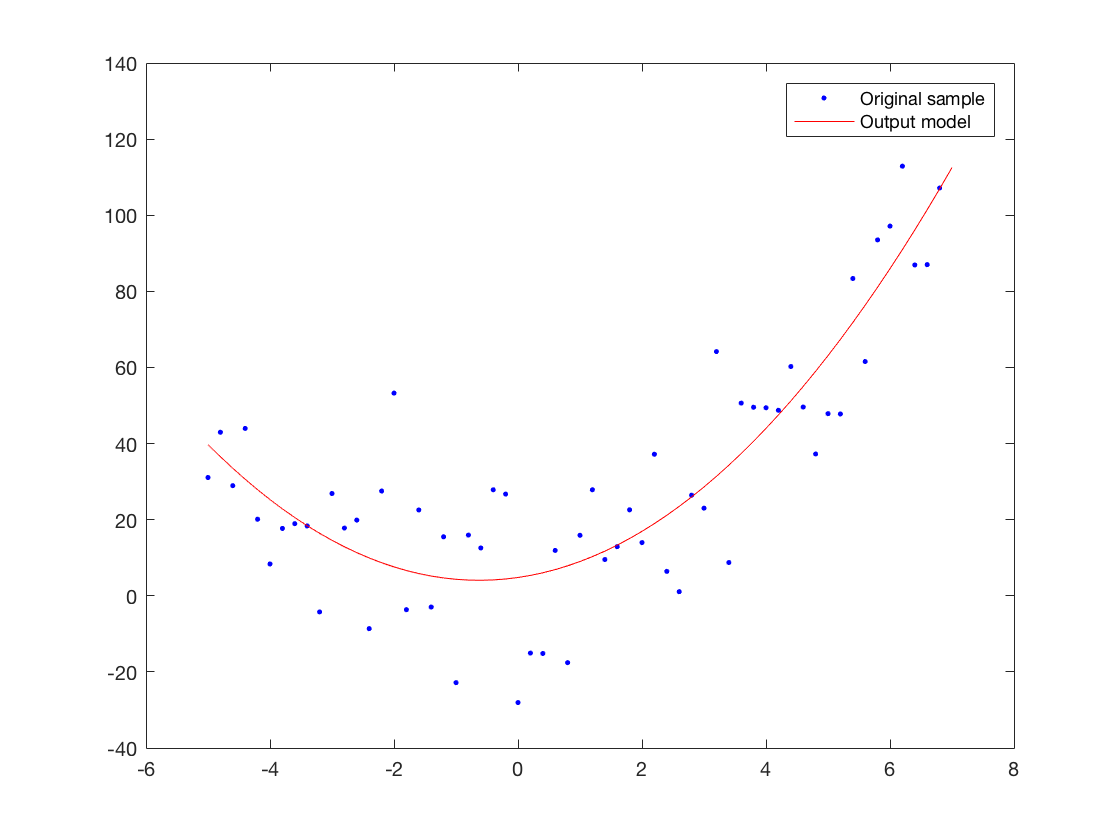
\includegraphics[width=0.7\textwidth]{1.png}
    \caption{Гистограмма и график функции плотности распределения нормальной случайной величины.}
\end{figure}



\newpage
\subsection{График эмпирической функции распределения и функции распределения нормальной случайной величины с математическим ожиданием $\hat{\mu}$ и дисперсией $S^2$}

\begin{figure}[h]
    \centering
    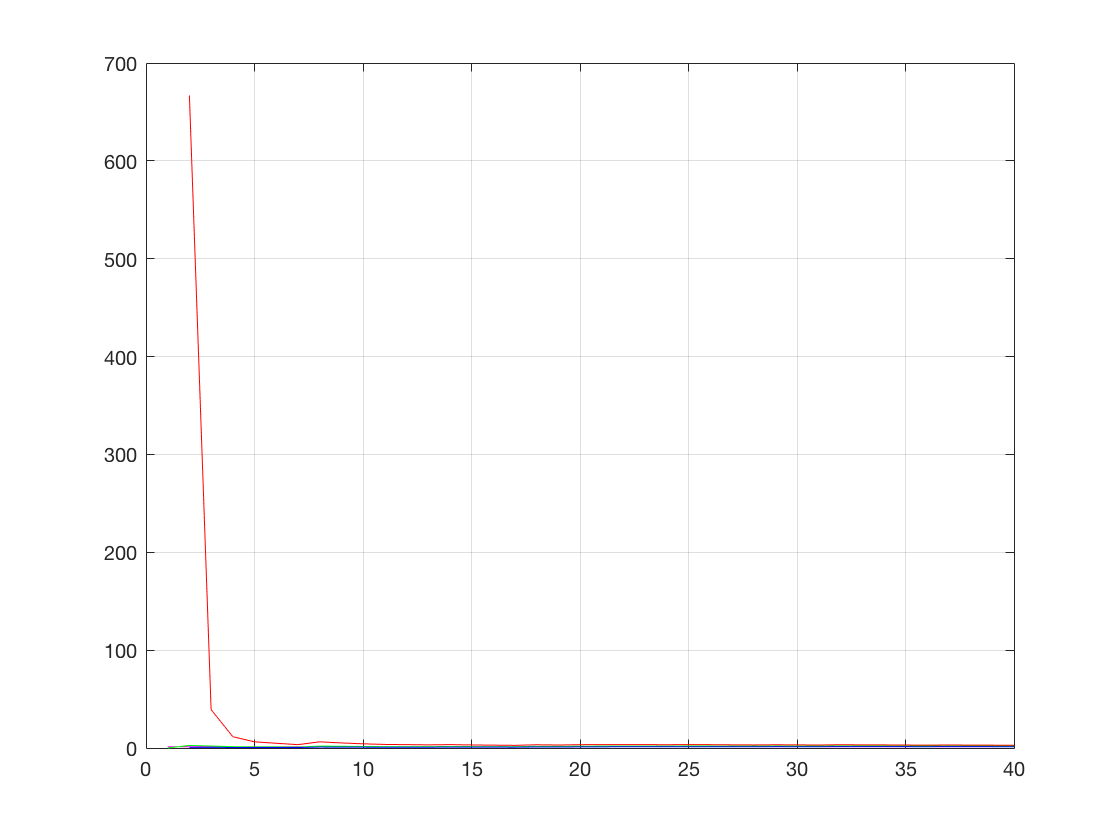
\includegraphics[width=0.7\textwidth]{2.png}
    \caption{График эмпирической функции распределения и функции распределения нормальной случайной величины.}
\end{figure}